\documentclass[conference]{IEEEtran}
\usepackage{blindtext, graphicx}
\usepackage{amsmath}
\usepackage{listings}


\ifCLASSINFOpdf
\else
\fi


% correct bad hyphenation here
\hyphenation{op-tical net-works semi-conduc-tor}


\begin{document}

% figures: only your own research
% paraphrases
% clearer statements related to the findings

\title{Chimera - Simple Language Agnostic Framework for Stand Alone and Distributed Computing}

\author{\IEEEauthorblockN{Go Frendi Gunawan}
\IEEEauthorblockA{STIKI Malang\\ Malang, Indonesia\\
Email: frendi@stiki.ac.id}
\and
\IEEEauthorblockN{Mukhlis Amien}
\IEEEauthorblockA{STIKI Malang\\
Malang, Indonesia\\
Email: amien@stiki.ac.id}
\and
\IEEEauthorblockN{Jozua Ferjanus Palandi}
\IEEEauthorblockA{STIKI Malang\\
Malang, Indonesia\\
Email: jozuafp@stiki.ac.id}}

% make the title area
\maketitle


\begin{abstract}
%\boldmath
Component-Based Software Engineering (CBSE) is a branch of software 
engineering that emphasizes the separation of concerns with respect to the 
wide-ranging functionality available throughout a given software system.  The 
main advantage of CBSE is separation of components. A single component  
only focus on a single task or a related collection of tasks which allowing software 
developer to reuse the component for other use-cases. By using this approach, 
spaghetti code is no longer used by software developers. Several 
approaches have already been developed in order to achieve ideal CBSE. The earliest 
implementation was UNIX pipe and redirect, while the newer approach including 
CORBA, XML-RPC, and REST. Therefore, a simple language-agnostic framework, 
so called Chimera, was developed in this research. Chimera was built on top of Node.js. 
This framework allows developer to build pipe flow in a chain (a YAML formatted file) 
as well as defining global variables. Compared to UNIX named and unnamed pipe, 
this format is easier and more flexible. On the other hand, unlike XML-RPC, 
REST, and CORBA, Chimera is much simpler. HTTP protocol is only required for
distributed computing scenario. Nor it require the components to be aware that 
they works on top of the framework.
\end{abstract}

% Note that keywords are not normally used for peerreview papers.
\begin{IEEEkeywords}
Chimera, Language Agnostic, Component-Based Software Engineering, CBSE, Node.js, CLI.
\end{IEEEkeywords}

\IEEEpeerreviewmaketitle

\section{Introduction}

Component-based software development approach is based on the idea of developing 
software systems by selecting appropriate off-the shelf components and then to 
assemble them with a well-defined software architecture \cite{kaur2010component}.

In order to implement Component-Based Software Engineering (CBSE), several 
approaches have been performed. The earliest attempt was UNIX pipe mechanism 
\cite{mcilroy1968mass}. Pipe mechanism was not the only attempt to achieve CBSE.
The more modern approaches including XML-RPC \cite{xmlrpc} and JSON-RPC \cite{jsonrpc}. 
Later, Object Management Group (OMG) introduced a new standard named CORBA (Common
Object Request Broker Architecture) \cite{corba}. Another interesting approach was 
introduced by Two Sigma Open Source. Two Sigma created a platform known as Beaker
Notebook \cite{beakernotebook} which is mainly used for research purposes. 
On 2016, Feilhauer and Sobotka introduce another platform called DEF 
\cite{feilhauer2016def}.

Despite Unix Pipe, the other mechanisms require the components to be aware that 
they are parts of the framework. It means that old programs (e.g.
{\it factor} and {\it calc}) as XML-RPC or CORBA component. At least, additional layer
and adjustment have to be built.

Moreover, CORBA, XML-RPC, SOAP, and JSON-RPC also need HTTP protocol since they were designed for 
client-server architecture. It imply that the developers need to build a web server for being able 
to use the mechanisms. However, in any use-case that only need a single computer,
this is not ideal.

Considering the advantages and disadvantages of earlier approaches, a new CBSE framework, 
named Chimera, was developed in this research. This framework is much simpler since
HTTP is required for distributed computation only. Chimera also use CLI mechanism that
works in almost all OS and in most programming language.
The only dependency of Chimera is Node.js and several NPM packages.

\section{Previous Research}

This section presents an in-depth discussion on the previous CBSE implementation,  
preceeding Chimera.


\subsection{UNIX Pipe}

The very first implementation of CBSE was UNIX pipe mechanism \cite{mcilroy1968mass} 
which allowed engineer to pass output of a single program as an input for 
another program. Since a lot of server was UNIX or linux based, this pipe 
mechanism availability was very high. Even, DOS also provide similar mechanism 
\cite{dos7command}.

Pipe mechanism work by allowing a program's standard output being used as another
program's standard input. By placing several programs into a single pipeline, 
a more complex process might be composed as depicted in figure ~\ref{fig:unixPipe}.

\begin{figure}
	\centering
	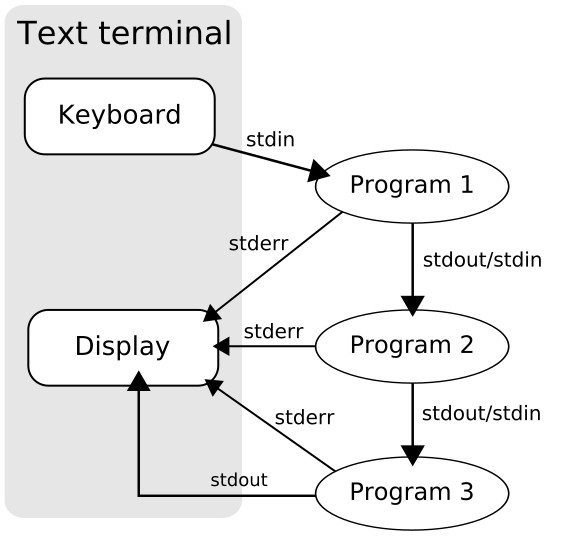
\includegraphics[width=0.3\textwidth]
		{images/Pipeline.jpg}
	\caption{Unix Pipeline Mechanism}
	\label{fig:unixPipe}
\end{figure}

For example, consider two different programs,
{\it factor} and {\it calc}. When a single argument is given, {\it factor} presents all 
factors of a number. Next, when a single argument is given, {\it calc} presents the result 
of an arithmetic operation. Listing ~\ref{factorAndCalc} depicts the output of both commands.

\begin{lstlisting}[caption=Usage of factor and calc, label=factorAndCalc, language=bash, basicstyle=\small, breaklines=true]
#! factor 20
20: 2 2 5

#! calc 7+3 
10
\end{lstlisting}

Unix pipe mechanism allows you to combine those two programs. For example, if you
want the output of {\it calc} become the input of {\it factor}, you can use pipe
command as shown in listing ~\ref{unnamedPipeExample}

\begin{lstlisting}[caption=Unnamed pipe example, label=unnamedPipeExample, language=bash, basicstyle=\small, breaklines=true]
#! calc 7+3 | factor
10: 2 5
\end{lstlisting}

Beside of its high availability and simplicity, UNIX pipe also supports parallel
processing through named-pipe mechanism. The named-pipe mechanism can be used to 
provide cheap parallel processing \cite{conway2003parallel}. As presented in 
listing ~\ref{namedPipeExample} a named pipe called {\it backpipe} was made by using {\it mkfifo} command. 
Then, the standard output of {\it calc} and {\it factor} is added into the {\it backpipe}. Finally, the content of the {\it backpipe} is presented using {\it cat} command.

\begin{lstlisting}[caption=Named pipe example, label=namedPipeExample, language=bash, basicstyle=\small, breaklines=true]
#! mkfifo backpipe 

#! calc 7+3 > backpipe | factor 20 > backpipe | cat backpipe
10
2 2 5
\end{lstlisting}

Although pipe mechanism provides high availability and capability, 
it has several limitations. For example, named-pipe mechanism needs external file, which has to be deleted once the operation performed, as a temporary container. This approach does not work straight forward, thus, some efforts needed in order to 
build a working named-pipe-based-computation. 

Pipe mechanism is suitable for simple use-cases involving a single computer. 
However, at some point, memory sharing  and network access are needed when the program become more complicated. 
Using a mere pipe mechanism to support those requirement needs a lot of 
efforts. Although it is possible, the readability of the script is severely reduced.


\subsection{CORBA}

From CORBA official website, CORBA is defined as standard created by the Object 
Management Group designed to facilitate the communication of systems 
that are deployed on diverse platforms \cite{corba}. CORBA 1.0 was released on August 
1991. The last version, CORBA 3.3, was released on November 2012 \cite{corbaspec}.
CORBA is heavily affected by object oriented paradigm.

The main component of CORBA is the Object Request Broker (ORB) which acts as a bridge 
between client and service provider. The service provider (server) provide an 
implementation of an object, while the client can be a user interface that depend on
the service provided by the server. Both, client and server need to agree about the
object structure. This agreement is written in an Interface Description Language (IDL),
the IDL which is called skeleton in server side, and is called stub in client side.

\begin{figure}
	\centering
	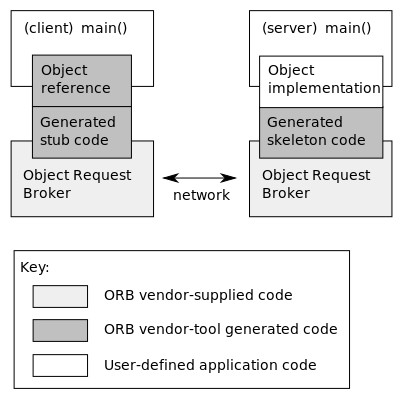
\includegraphics[width=0.3\textwidth]
		{images/Orb.jpg}
	\caption{Object Request Broker}
	\label{fig:orb}
\end{figure}

IDL can be written in Java, C++, or any other language, depending on the implementation of
the ORB. An IDL example is shown in listing ~\ref{corbaIDLExample}. 
The interaction between ORB, server, and client depicts in figure ~\ref{fig:orb}.
 
\begin{lstlisting}[caption=CORBA IDL Example in C++, label=corbaIDLExample, language=c, basicstyle=\small, breaklines=true]
module Finance {
  typedef sequence<string> StringSeq;
  struct AccountDetails {
    string     name;
    StringSeq  address;
    long       account_number;
    double     current_balance;
  };
  exception insufficientFunds { };
  interface Account {
    void deposit(in double amount);
    void withdraw(in double amount) raises(insufficientFunds);
    readonly attribute AccountDetails details;
  };
};
\end{lstlisting}

Compared to UNIX Pipe, CORBA has more complex and rich features. Unfortunately, this also means 
that CORBA is also more complex than UNIX Pipe. The developer needs to embrace OOP 
paradigm as well as being familiar with IDL and the CORBA architecture. 
Despite of it's language agnoticism, some non OOP language (e.g: Matlab and GNU Octave) 
is not supported by CORBA \cite{feilhauer2016def}. CORBA also suffers of several 
criticism \cite{henning2006rise}. Regardless to it's popularity, there are many critics towards OOP, 
as the foundation of CORBA \cite{hadar2013intuition}.


\subsection{XML-RPC, SOAP, and JSON-RPC}

XML-RPC is a specification and a set of implementations that allows software running on 
disparate operating systems and in different environments to make procedure 
calls over the Internet. XML-RPC use HTTP as the transport and XML as the encoding.
It is designed to be as simple as possible, meanwhile it allows complex data structures to 
be transmitted, processed and returned \cite{xmlrpc}. SOAP stands for Simple Object Access Protocol. 
SOAP is a lightweight protocol intended for exchanging structured information in a decentralized, distributed 
environment \cite{soap}. SOAP was built on top of XML-RPC. It uses XML format as 
well as HTTP protocol.

JSON-RPC is lightweight remote procedure call protocol similar to XML-RPC 
\cite{jsonrpc}. The main difference between XML-RPC and JSON-RPC is the data transfer
format. In most cases, JSON is more lightweight compared to XML.

XML-RPC, SOAP, and JSON-RPC heavily depend on HTTP for their inter-process-communication 
protocol. This is ideal for client-server architecture as HTTP is quite common and
easy to be implemented. Those three methods are basically another implementation of RPC (Remote Procedure Call). 
Compared to CORBA, these three methods are more flexible. With the exception of SOAP,
they don't enforce developer to embrace OOP paradigm.

In terms of language agnoticism, XML-RPC and JSON-RPC support any languages that can
access HTTP and parse/create the data format. However, in order to use these protocols,
a developer should be aware that the components they built work as a part of a
bigger system. Tools or programs that built without this consideration need
some adjustments or additional layers in order to make them work with the protocol.
For example, using {\it{factor}} or {\it{calc}} as components of XML-RPC might require
developer to build another program to catch the output and wrap it in XML envelope.

\subsection{DEF}

DEF is a programming language agnostic framework and execution environment 
for the parallel execution of library routines \cite{feilhauer2016def}. 
DEF focuses on parallel processing by enabling shared memory and message passing. 
DEF needs several components and so JSON as data exchange format. 
DEF is better in terms of parallelism and language agnosticism compared to CORBA, Matlab, and Parallel Fortran. 
CORBA for example, doesn't support matlab and octave \cite{feilhauer2016def}. 

However, DEF still depends on HTTP for inter-process communication. Consequently, 
in order to build DEF architecture, a web server is needed. Also, the developer needs 
to make sure that each components aware of the architecture. As in CORBA, XML-RPC, 
SOAP, and JSON-RPC, additional layer might be needed to make use of old components.

\subsection{Beaker Notebook}

Beaker Notebook \cite{beakernotebook} is also considered as an interesting 
approach of CBSE. The platform was developed by Two Sigma Open Source 
for research purposes only. Beaker Notebook provides native autotranslation that 
lets a developer declare specific variables in a cell in one language, 
and access them seamlessly in a different cell and language.

Llisting ~\ref{beakerPython} describes a 6 by 4 table populated with
random numbers. The table is, then, saved as global variable df. 
The data is loaded and showed in listing ~\ref{beakerR}.

\begin{lstlisting}[caption=Beaker Python Cell Example, label=beakerPython, language=python, basicstyle=\small, breaklines=true]
import pandas
beaker.df = pandas.DataFrame(np.random.randn(6, 4), columns = list('ABCD'))
\end{lstlisting}

\begin{lstlisting}[caption=Beaker R Cell Example, label=beakerR, language=R, basicstyle=\small, breaklines=true]
beaker::get('df')
\end{lstlisting}

Moreover, Beaker Notebook is good for prototyping. It also has a very simple API compared to
CORBA or XML-RPC. However, it still require the developer to add additional layer
in order to use old components like {\it factor} or {\it calc}


\section{Chimera Architecture}

From the previous section, it can be concluded that Unix Pipe Mechanism was the simplest one
despite of it's lack of features. We also notice that Beaker Notebook's like memory-
sharing mechanism is much simpler compared to CORBA and other network-based protocols.

The objective of this research is to make a very simple framework that is truly language agnostic. The framework
should be able to accomodate with old components and should not enforce developers to embrace any 
particular programming paradigms. Moreover, making unnecessary new standard is avoided in this research.
By making use of technologies that most developers are familiar with, it is expected that the adaptation is
going to be easier. It is assumed that most programming languages supports command line interface and
command line arguments. By creating a framework that depends on command line protocol,
maximum language agnosticism with less effort is achieved.

In figure ~\ref{fig:chimeraArchitecture} we show the architecture of Chimera. Suppose
{\it Program1} and {\it Program2} should run in parallel, and {\it Program3} should be
executed once {\it Program1} and {\it Program2} finished.

Chimera architecture consists of several parts. The Chimera Core is the main component 
that responsible for orchestrating external programs into a single process flow. 
Chimera Core can access temporary memory which is no other than a JSON Object placed in
memory. All input and output of external programs are copied into this JSON Object.
The process flow itself written in a YAML Chain File. YAML is a common format for
configuration. YAML depends on indentation and whitespace, making the format easily 
readable. Using these three components, Chimera is able to do everything that UNIX Pipe is able to do. 
In fact, developers can even define the UNIX Pipe inside Chimera. The other two components are Chimera-Service and Chimera-Sender. These two components are responsible for HTTP communication. Chimera-Service and Chimera-Sender brings the 
entire framework into distributed environment.

Figure ~\ref{fig:chimeraArchitecture} describes the process started when the user ask Chimera 
to execute the process. User should provides the YAML file location and the process
inputs. After getting a request from user, Chimera read the YAML file, retrieving
content, and initiating global variables in temporary memory. The framework, then,
executes external programs sequentially or parallel, depending on the content of the
YAML file. When the external programs are located in the same computer, Chimera-Core executes the
programs and provides the required stdin parameters which are taken from
temporary memory. After the program executed successfully, Chimera-Core  reads the 
stdout and saves it in the temporary memory for further process.

In case the programs are located in different computer, the user should provide
invocation of Chimera-Sender then Chimera-Sender contacts Chimera-Service to run 
Chimera-Core remotely. Once the process completed, Chimera-Service sends 
response back to Chimera-Sender. At last, Chimera-Sender sends the response back to
the local Chimera-Core.

At the end of the process, Chimera returns the output of those chain-processes to 
the user.

\begin{figure*}
	\centering
	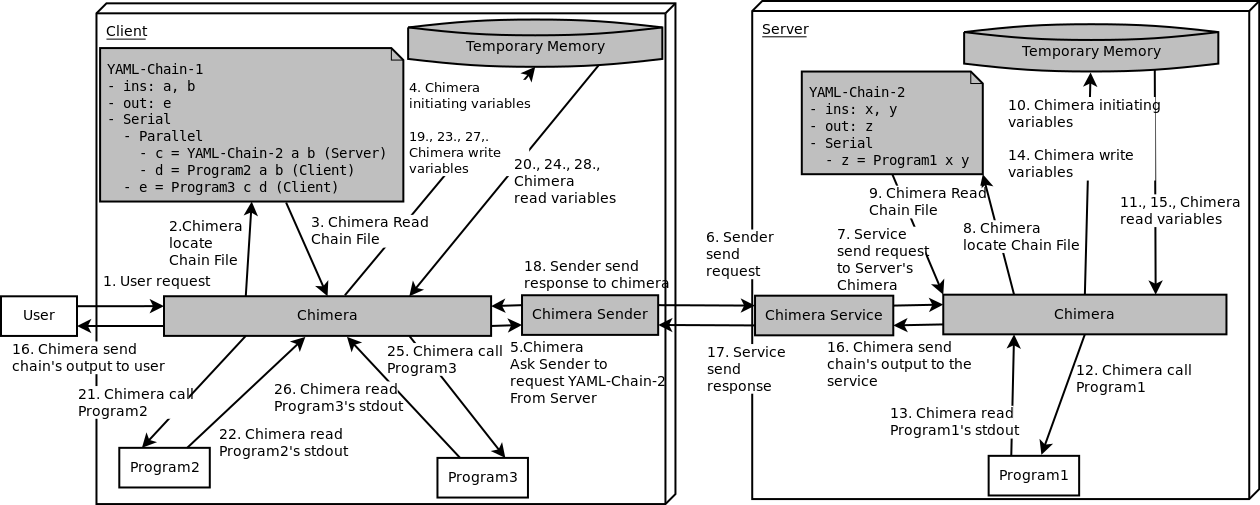
\includegraphics[width=1.0\textwidth]
		{images/chimera.png}
	\caption{Architecture of Chimera}
	\label{fig:chimeraArchitecture}
\end{figure*}

\section{Chimera Technical Implementation}

Chimera as an NPM package has been published and accessible at 
https://www.npmjs.com/package/chimera-framework.


\subsection{Node.js and NPM As Chimera's Foundation}

Chimera was written in Node.js. Node.js itself is a JavaScript runtime built on Chrome 
V8 JavaScript engine. Node.js uses an event-driven, a non-blocking I/O model that makes it 
lightweight and efficient \cite{nodejs}. Compared to Python and PHP, Node.js has an 
overall better performance \cite{lei2014performance}. Node.js is also available for
Windows, Linux, and Mac.

Node.js has a package-manager named NPM (Node Package Manager). This allows developers
to use libraries that have already been written by other developers. Chimera depends on 
several packages:

\begin{itemize}
    \item async
    \item express
    \item fs-extra
    \item http
    \item js-yaml
    \item node-cmd
    \item path
    \item process
    \item querystring
\end{itemize}

Async package was used to develop the control flow since Node.js has non-blocking
mechanism. Express which allows us to catch request
and to send appropriate response was used to build Chimera-Service. Fs-extra was also used in order to do file operations.
Http and querystring were used to build Chimera-Sender. Several functionalities
provided by node-cmd were needed in order to execute other programs through CLI mechanism.
Js-yaml was used for YAML parsing. At last, path and process were needed to determine 
absolute path of a file as well as to change directory and retrieve input arguments.

\subsection{YAML for Defining Chain}

YAML (YAML Ain't Markup Language) standard, when was built in 2001, is a human friendly data serialization standard for 
all programming languages \cite{yaml}. Unlike JSON,
YAML depends heavily on indentation. Although its size is bigger compared to JSON, YAML
is readable and commonly used for configuration.

At first, Chimera's chain file was intended to use JSON format. However, the use of JSON format might not be a good decision since the developers have to be very 
careful with commas and curly braces. Another disadvantage
of JSON is that it doesn't provide any intuitive way to add comments, which is quite
essential in writing algorithms.

Let consider having several programs written in Python, Java, PHP, and Javascript. 
Each of them takes two arguments, does simple arithmetic operation, and return a single output. 
Given a and b, to be calculated ((a+b) * (a-b)) + a.

The process csan be written as follow:

{\it f = ((a+b) * (a-b)) + a}

Then, this process is divided into several sub-processes:

\begin{itemize}
    \item Process 1: c = a + b
    \item Process 2: d = a - b
    \item Process 3: e = c * d
    \item Process 4: f = e + a
\end{itemize}

Process 1 and process 2 are executed parallelly since they are independent to each other. 
It is not necessary to solve process 1 first in order to do process 2 and vice versa.

After process 1 and process 2 finished, process 3 and process 4 should be executed sequentially. 
Process 3 depends on process 1 and 2, while process 4 depends on process 3

Listing ~\ref{yamlChainExample} is the example of YAML formatted chain file.

\begin{lstlisting}[caption=YAML Chain Example, label=yamlChainExample, language=yaml, basicstyle=\small, breaklines=true]
ins: a,b # The inputs of main process 
out: f # The outputs of main process 
series:
  # Process 1 and 2 
  - parallel:
      # Process 1 (in Python) 
      - ins: a, b
        out: c
        command: python programs/add.py
      - series: # Process 2 (in Java) 
          # First, compile the source  
          - javac programs/Substract.java
          # then run the program 
          - ins: a, b
            out: d
            command: java -cp programs Substract
  # Process 3 (in PHP) 
  - ins: c, d
    out: e
    command: php programs/multiply.php
  # Process 4 (in Javascript) 
  - ins: e, a
    out: f
    command: node programs/add.js
\end{lstlisting}

Similar to other programs, semantically, each node in YAML contains {\it ins} and {\it out } which means that the program might have more than one inputs but it only provide one single output. 
The last element of the node is either {\it command}, {\it parallel}, or {\it series}. 
If the process has no other sub-process, {\it command} is used. Otherwise, if the
process contains another sub-process, {\it parallel} or {\it series} is used depending
on the desired execution flow. The best practice is that parallel flow is recommended, when two or more processes
are independent on each other. Listing  ~\ref{yamlShort} provides single-line shorthand for {\it ins}, {\it out}, 
and {\it command}. {\it ins} should be written inside parantheses, while {\it ->}
act as separator between {\it ins}, {\it command}, and {\it output}. 
Listing  ~\ref{yamlShort} is equal to Listing ~\ref{yamlChainExample}.

\begin{lstlisting}[caption=YAML Chain With Shorthand, label=yamlShort, language=yaml, basicstyle=\small, breaklines=true]
ins: a,b # The inputs of main process 
out: f # The outputs of main process 
series:
  # Process 1 and 2 
  - parallel:
      # Process 1 (in Python) 
      - (a,b) -> python programs/add.py -> c
      - series: # Process 2 (in Java) 
          # First, compile the source  
          - javac programs/Substract.java
          # then run the program 
          - (a,b) -> java -cp programs Substract -> d
  # Process 3 (in PHP) 
  - (c,d) -> php programs/multiply.php -> e
  # Process 4 (in Javascript) 
  - (e,a) -> node programs/add.js -> f
\end{lstlisting}


\subsection{JSON Format for Temporary Global Storage and Data Transfer}

When Node.js is used, it is common to use Javascript Object Notation as Chimera's
global storage and network data transfer. JSON (JavaScript Object Notation) is a 
lightweight data-interchange format \cite{json}. Once the YAML Chain File parsed, Chimera creates several variables in {\it name : 
value} pairs. For example, after loading YAML in Listing ~\ref{yamlChainExample}, the
global variables contain JSON object as shown in Listing ~\ref{jsonStorageInitial}. As the sub-process executed, several others variables will be added as needed. At the
end of the process, the global storage contains a, b, c, d, e, and f.

\begin{lstlisting}[caption=Initial content of JSON Storage, label=jsonStorageInitial, language=json, basicstyle=\small, breaklines=true]
{
    "a" : 0,
    "b" : 0,
    "f" : 0,
}
\end{lstlisting}

Not only for temporary storage, we also use JSON for data transfer between 
Chimera-Sender and Chimera-Service. The data sent to Chimera-Service is shown in Listing
~\ref{jsonRequest}, while the data received by Chimera-Sender is shown in Listing
~\ref{jsonResponse}.

The JSON request contains two keys, i.e. the "chain" for 
indicating the remote YAML chain file location and "input" containing array of inputs.

Meanwhile, the JSON response contains three keys, i.e. the {\it success} key for indicating
whether the request succeed or failed, {\it errorMessage} containing the error message and
{\it response} is the response from the server.

\begin{lstlisting}[caption=JSON Request, label=jsonRequest, language=json, basicstyle=\small, breaklines=true] 
{
    "chain" : "remote-chain-file.yaml",
    "input" : [],
}
\end{lstlisting}

\begin{lstlisting}[caption=JSON Response, label=jsonResponse, language=json, basicstyle=\small, breaklines=true]
{
    "success" : true,
    "errorMessage" : "",
    "response" : "",
}
\end{lstlisting}


\subsection{Utilities}

Several utilities were built as the components of Chimera Framework, such as:

\begin{itemize}
    \item Chimera-core
    \item Chimera-eisn
    \item Chimera-serve
    \item Chimera-send
\end{itemize}

Chimera-core is the main component of the framework in which user can invoke Chimera by
executing {\it chimera your-chain-file.yaml [input1 [input2] ... ]}. In terms of convenience,
some shorthands are also provided, e.g. the use of chimera 
{\it chimera "command:cal"} or even {\it chimera "cal"} to call Chimera.

Chimera-eisn takes at least three input arguments. The first and the second argument should
be file name, while the third arguments should be the command. The command is 
executed only when the first argument's modification date is newer than the second 
argument. EISN itself stands for "Execute If Source Newer". This is useful when a user
wants to use source code of compiled language as an argument as described in Listing ~\ref{chimeraEisn}

\begin{lstlisting}[caption=Chimera-eisn usage example, label=chimeraEisn, language=yaml, basicstyle=\small, breaklines=true]
ins: a, b
out: c
series:
    - chimera-eisn add.java add.class javac add
    - ins: a, b
      out: c
      command: java add
\end{lstlisting}

Chimera-serve is a utility to allow several chain files being served by a computer.
The typical usage of chimera-serve is:

{\it TIMEOUT=5000 PUBLISHED=. chimera-serve}

The first two statements are used to define timeout and to publish directory. Dot means
current directory. All chain files in published directory are accessible over the network.

Chimera-send is a utility to access chimera service.
The typical usage of chimera-send is: 

{\it TIMEOUT=5000 chimera-send remoute-chain-file.yaml [input1 [input2] ... ]}


\section{Test}

Listing ~\ref{distributedParallelYaml} describes the process of testing whether the Chimera works
in parallel and distributed environment.

\begin{lstlisting}[caption=Distributed and Parallel YAML-chain Scenario, label=distributedParallelYaml, language=yaml, basicstyle=\small, breaklines=true]
ins: a,b,server
out: e
vars:
  server_chain: tests/chain-minimal.yaml 
verbose: true
series:
  - parallel:
      # Process 1
      - (a,b) -> php programs/add.php -> c
      # Process 2
      - (server, server_chain, a,b) -> chimera-send -> d
  # Process 3
  - (c,d) -> node programs/add.js -> e
\end{lstlisting}

The chain consisted of three processes. Process 1 and process 2 was executed in parallel.
After process 1 and process 2 finished, process 3 was executed. Unlike process 1 and
process 3, process 2 will ran on the server.

On the server side, {\it chimera-serve} was executed so that it was able to listen the client's request
and to give response as necessary.

Meanwhile, on the client side, it was executed at {\it chimera tests/chain-distributed.yaml 4 5 http://localhost:3000}. The client log depicts in listing ~\ref{clientLog} 

\begin{lstlisting}[caption=Client Log, label=clientLog, language=bash, basicstyle=\small, breaklines=true]
START [php programs/add.php "4" "5"] AT    : 15,395,587,568,188
START [chimera-send "http://localhost:3000" "tests/chain-minimal.yaml" "4" "5"] AT    : 15,395,607,233,624
END   [php programs/add.php "4" "5"] AT    : 15,395,641,517,534
TAKES 53,905,697 NS
END   [chimera-send "http://localhost:3000" "tests/chain-minimal.yaml" "4" "5"] AT    : 15,396,103,823,215
TAKES 496,566,143 NS
START [node programs/add.js "9" "-5"] AT    : 15,396,105,155,463
END   [node programs/add.js "9" "-5"] AT    : 15,396,187,724,022
TAKES 82,541,434 NS
4
\end{lstlisting}

From the log, it can be seen that the second process on client side was executed before the first process finished.
However, the third process didn't start before the second process started. The output of process 2  was taken from the
server's response.


\begin{figure}
	\centering
	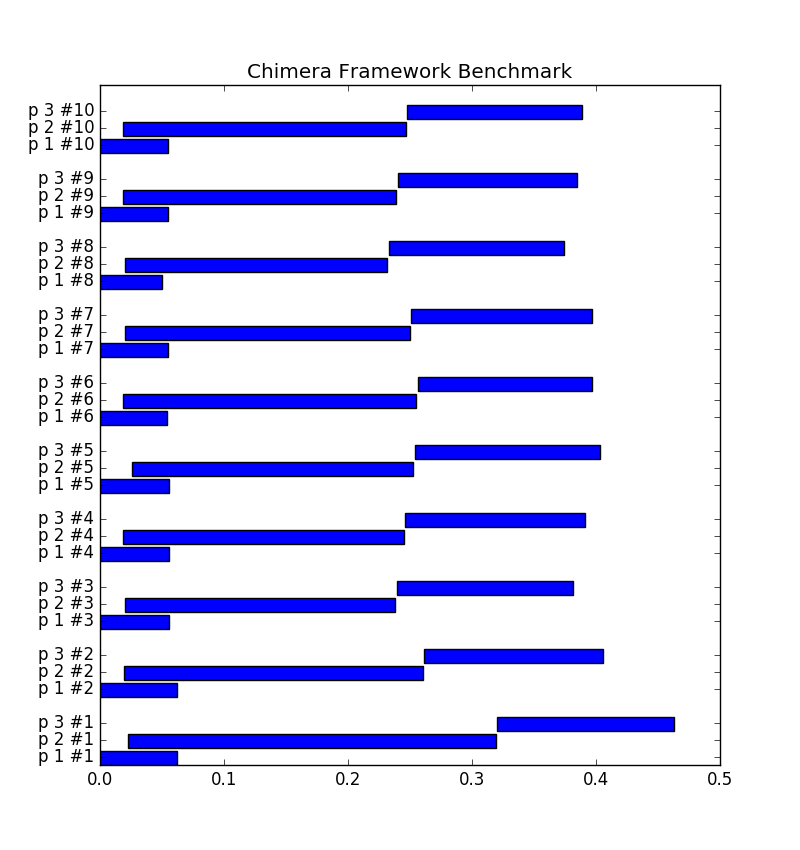
\includegraphics[width=0.5\textwidth]
		{test/report.png}
	\caption{Test}
	\label{fig:test}
\end{figure}

\section{Conclusion}

Chimera, a simple language agnostic CBSE Framework has been developed in this research. The framework is quite simple, yet powerful enough for being used on distributed and parallel computation.

Old UNIX commands, like {\it calc} and {\it factor}, work perfectly as well under the framework and
no additional layer needed.

%\appendices
%\section{Proof of the First Zonklar Equation}

% use section* for acknowledgement
\section*{Acknowledgment}

The authors would like to thank Sonny Setiawan, Satriyo Wibowo, Dani Devito, and Zusana Pudyastuti for their suggestions and inputs.

% Can use something like this to put references on a page
% by themselves when using endfloat and the captionsoff option.
\ifCLASSOPTIONcaptionsoff
  \newpage
\fi

\bibliographystyle{IEEEtran}
\bibliography{./citation}

% that's all folks
\end{document}

